%%%%%%%%%%%%%%%%%%%%%%%%%%%%%%%%%%%%%%%%%%%%%%%%%%%%%%%%%%%%%%%%%%%%%%%%%%%%%%%%
%2345678901234567890123456789012345678901234567890123456789012345678901234567890
%        1         2         3         4         5         6         7         8

\documentclass[letterpaper, 10 pt, conference]{ieeeconf}  % Comment this line out if you need a4paper

%\documentclass[a4paper, 10pt, conference]{ieeeconf}      % Use this line for a4 paper

\IEEEoverridecommandlockouts                              % This command is only needed if 
                                                          % you want to use the \thanks command

\overrideIEEEmargins                                      % Needed to meet printer requirements.
\pdfminorversion=4

% See the \addtolength command later in the file to balance the column lengths
% on the last page of the document

% The following packages can be found on http:\\www.ctan.org
\usepackage{graphics} % for pdf, bitmapped graphics files
%\usepackage{epsfig} % for postscript graphics files
%\usepackage{mathptmx} % assumes new font selection scheme installed
%\usepackage{times} % assumes new font selection scheme installed
\usepackage{amsmath} % assumes amsmath package installed
\usepackage{amssymb}  % assumes amsmath package installed
\usepackage{graphicx}
\usepackage{subfigure}
\usepackage{epstopdf}
\usepackage{threeparttable}

% Some handy commands
\newcommand{\norm}[1]{\left\Vert#1\right\Vert}
\newcommand{\abs}[1]{\left\vert#1\right\vert}
\newcommand{\set}[1]{\left\{#1\right\}}
\newcommand{\Real}{\mathbb R}
\newcommand{\Complex}{\mathbb C}
\newcommand{\eps}{\varepsilon}
\newcommand{\To}{\longrightarrow}
\newcommand{\Ker}{\textup{Ker}}
\newcommand{\Img}{\textup{Img}}
\newcommand{\diag}{\textup{diag}}
\newcommand{\circulant}{\textup{circ}}
\newcommand\T{\rule{0pt}{2.6ex}}        % Top strut
\newcommand\B{\rule[-1.2ex]{0pt}{0pt}} % Bottom strut

% Custom math defs
\def\Vec#1{\mathbf{#1}}
\newcommand{\bbm}{\begin{bmatrix}}
\newcommand{\ebm}{\end{bmatrix}}
\DeclareMathAlphabet{\mbf}{OT1}{ptm}{b}{n}
\newcommand{\mbs}[1]{{\boldsymbol{#1}}}
\newcommand{\pd}[2]{\frac{\partial #1}{\partial #2}}

\title{\LARGE \bf
The Battle for Filter Supremacy: A Comparative Study of the Multi-State Constraint Kalman Filter and Sliding Window Filter
}


\author{Lee Clement$^{1}$ and Valentin Peretroukhin$^{1}$% <-this % stops a space
%\thanks{*This work was not supported by any organization}% <-this % stops a space
\thanks{$^{1}$Institute for Aerospace Studies,
        University of Toronto, Toronto, ON, Canada
        {\tt \{lee.clement, valentin.peretroukhin\} @robotics.utias.utoronto.ca}
        }%
}

\begin{document}



\maketitle
\thispagestyle{empty}
\pagestyle{empty}


%%%%%%%%%%%%%%%%%%%%%%%%%%%%%%%%%%%%%%%%%%%%%%%%%%%%%%%%%%%%%%%%%%%%%%%%%%%%%%%%
\begin{abstract}
Accurate and consistent egomotion estimation is an important part of autonomous vehicles. The combination of visual and inertial sensors provides a relatively inexpensive, compact and complementary hardware suite that can be used on many ground and aerial vehicles. In this work, we compare two modern approaches to egomotion estimation: the Multi-State Costraint Kalman Filter (MSCKF) and the Sliding Window Filter (SWF). Both filters use an Inertial Measurement Unit (IMU) to estimate the motion of a monocular camera and then correct this motion with image observations of salient features. The SWF includes the feature positions in the state estimate itself, while the MSCKF estimates the feature positions in a separate optimization routine. Herein, we compare the performance of the MSCKF and SWF, in error bounds and consistency, on two different datasets with real and synthetic features. We analyze the effect of feature track length and feature density. In general, the SWF is found to be more accurate than the MSCKF. The MSCKF, however, is signficantly faster to compute, has good consistency, and its performance improves with more tracked features. 
\end{abstract}


%%%%%%%%%%%%%%%%%%%%%%%%%%%%%%%%%%%%%%%%%%%%%%%%%%%%%%%%%%%%%%%%%%%%%%%%%%%%%%%%
\section{INTRODUCTION} \label{sec:introduction}

The combination of visual and inertial sensors is a powerful tool for autonomous navigation in unknown environments.
Indeed, cameras and inertial measurement units (IMUs) are complementary in several respects.
Since an IMU directly measures accelerations and rotational velocities, these values must be integrated to arrive at a new pose estimate.
However, the noise inherent in the IMU's measurements is included in the integration as well, and consequently the pose estimates can drift unbounded over time.
The addition of a camera is an excellent way to bound this cumulative drift error since the camera's signal-to-noise ratio is highest when the camera is moving slowly.
On the other hand, cameras are not robust to motion blur induced by large accelerations.
In these cases, the strength of the IMU's signal far exceeds its baseline noise and can be relied upon more heavily in estimating pose changes.

The question, then, is how best to fuse measurements from these two sensor types to arrive at an accurate estimate of a vehicle's motion over time.
A complicating factor in the general form of this problem is the absence of a known map of features from which the camera can generate measurements.
Any solution must therefore solve a Simultaneous Localization and Mapping (SLAM) problem, although the importance placed on the mapping component may vary from algorithm to algorithm.

In this work, we compare and contrast three modern solutions, the Extended Kalman Filter (EKF), the Sliding Window Filter (SWF), and a hybrid solution, the Multi-State Constraint Kalman Filter (MSCKF) \cite{Mourikis:2006:TechReport,Mourikis:2007:ICRA}, that combines the strengths of both.
We present an experimental comparison of the SWF and MSCKF using a dataset consisting of IMU and camera data with accurate ground truth for both sensor motion and landmark positions.

%%%%%%%%%%%%%%%%%%%%%%%%%%%%%%%%%%%%%%%%%%%%%%%%%%%%%%%%%%%%%%%%%%%%%%%%%%%%%%%%
\begin{figure}
    \centering
    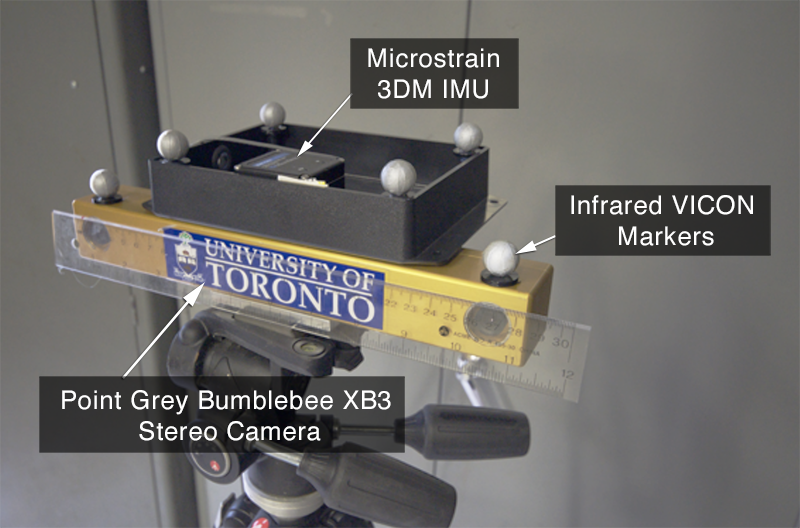
\includegraphics[width=0.45\textwidth]{figs/sensorhead}
    \caption{The sensor head used in our experiments. The IMU measures translational and rotational velocities, while the stereo camera measures the positions of point features. In our experiments, we artificially blinded the stereo camera by using measurements from the left camera only.}
    \label{fig:sensorhead}
\end{figure}

\section{Extended Kalman Filter (EKF)} \label{sec:EKF}
In the Extended Kalman Filter (EKF) solution, vehicle poses and feature positions are simultaneously estimated at each time step by augmenting the filter state with feature positions.
This technique, sometimes referred to as EKF-SLAM, attempts to track pose changes and create a globally consistent map of features by recursively updating the state as new measurements become available.
%Features are commonly parametrized as three-dimensional vectors and are initialized using two-view geometry, but alternative parametrization and initialization schemes exist \cite{Sola:2011:IJCV}.
%In this paper we consider only the three-dimensional parametrization and two-view initialization scheme.

Although the recursive nature of EKF-SLAM allows it to operate online, the computational cost of the filter grows cubically with map size.
This behavior is due to the fact that the dimension of the state grows linearly with the number of features, and the computational cost of inverting the state covariance matrix while computing the Kalman gain is cubic in the dimension of the state.
Consequently, the spatial extent over which EKF-SLAM can be used online is limited by the necessarily finite compute envelope available to it.

Another limitation of EKF-SLAM is that it is forgetful.
Because the filter state includes only the most recent vehicle pose, a given update step can never modify past poses even if later feature measurements ought to constrain them.
By locking in past poses, the EKF-SLAM formulation condemns itself to sub-optimally estimating both vehicle motion and feature positions.

%%%%%%%%%%%%%%%%%%%%%%%%%%%%%%%%%%%%%%%%%%%%%%%%%%%%%%%%%%%%%%%%%%%%%%%%%%%%%%%%
\section{Sliding Window Filter (SWF)} \label{sec:SWF}
In contrast to EKF-SLAM, the aim of the Sliding Window Filter (SWF) is not to construct a globally consistent map, but rather to estimate a vehicle's motion by optimizing a sliding window of vehicle poses and feature positions.
The optimization problem in the SWF is typically solved as a non-linear least squares problem using Gauss-Newton optimization or some other algorithm.
\begin{equation}
(\Vec H^T \Vec T ^{-1} \Vec H ) \delta \Vec{x}^*  = - \Vec{H}^T\Vec{T}^{-1}\Vec{e}(\bar{\Vec{x}})
\end{equation}
\begin{equation}
\delta\Vec{x} := \bbm \delta \Vec x_0 & \hdots & \delta \Vec x_K & \delta \Vec f_1 & \hdots & \delta \Vec f_N\ebm ^T,
\end{equation}
where $N$ is the number of unique features observed in the window.
The matrix $\Vec{H}$ is given by (showing non-zero blocks only)
\begin{equation}
\mathbf{H} = \left[\begin{array}{cccccc}
 -\Vec H_{\Vec x, 1} & \Vec 1 & &  & &   \\ 
 & -\Vec G_{\Vec x, 1} &  &  &  &   -\Vec G_{\Vec f, 1} \\ \hline
 & -\Vec H_{\Vec x, 2} & \Vec 1 & & &    \\ 
 & & -\Vec G_{\Vec x, 2} &  & &  -\Vec G_{\Vec f, 2}   \\ \hline
 &  & \ddots & \ddots & & \vdots  \\  \hline
  & & & -\Vec H_{\Vec x, K} & \Vec 1 & \\ 
 & & & & -\Vec G_{\Vec x, K} &  -\Vec G_{\Vec f, K}   \\  
\end{array}\right], 
\end{equation}
where
\begin{align}
\Vec G_{\Vec{x}, k}^j &= \pd{\Vec g}{ \Vec p}\Bigr|_{\bar{\Vec p}_{C_k}^{f_j C_k}}
    \bbm -\Vec C_{CG} \Vec C_{IG,k} \\[0.5em] \Vec C_{CG} (\Vec C_{IG,k} (\boldsymbol{\rho}_i^{f_j G} - \Vec r_G^{IG,k} ) )^\times  \ebm ^T
\\[0.5em]
\Vec G_{\Vec x, k} &= \bbm \Vec G_{\Vec x, k}^1 & \hdots & \Vec G_{\Vec x, k}^M \ebm ^T
\\[0.5em]
\Vec G_{\Vec f, k}^j &= \pd{\Vec g}{ \Vec p}\Bigr|_{\bar{\Vec p}_{C_k}^{f_j C_k}} \Vec C_{CI} \Vec C_{IG,k}
\\[0.5em]
\Vec G_{\Vec f, k} &= \underbrace{\bbm \Vec G_{\Vec f, k}^1 & & \\ & & \Vec G_{\Vec f, k}^2 & \\ & & \vdots &  \\ & & & \Vec G_{\Vec f, k}^M \ebm}_{\text{$j$th block column position given by feature ID $j$}}
\end{align}
with
\begin{equation}
\bar{\Vec p}_{C_k}^{f_j C_k} := \bbm x \\ y \\ z \ebm = \Vec C_{CI} \left( \Vec C_{IG,k} (\boldsymbol{\rho}_G^{f_j G} - \Vec r_G^{IG,k} )   - \boldsymbol \rho_I^{CI} \right),
\end{equation}

\begin{equation}
\pd{\Vec g}{ \Vec p}\Bigr|_{\bar{\Vec p}_{C_k}^{f_j C_k}} = \frac{1}{z^2} \bbm f_u z & 0 & - f_u x \\  0 & f_v z & -f_v y \ebm.
\end{equation}



An important advantage of the SWF is that its computational cost depends on the number of features in the current window rather than the number of features in the entire map.
By varying the spatial or temporal extent of the sliding window, the computational cost of the algorithm can be tailored to fit a given compute envelope, which makes the algorithm suitable for online operation over paths of arbitrary length.

However, the hard cut-off of the SWF may result in only some measurements of a particular feature contributing to the optimization.
As a result, the filter may not maximally constrain some vehicle poses, and hence localization may be less accurate than we could expect from the full batch solution.

%%%%%%%%%%%%%%%%%%%%%%%%%%%%%%%%%%%%%%%%%%%%%%%%%%%%%%%%%%%%%%%%%%%%%%%%%%%%%%%%
\section{MULTI-STATE CONSTRAINT KALMAN FILTER} \label{sec:MSCKF}
The Multi-State Constraint Kalman Filter (MSCKF) \cite{Mourikis:2006:TechReport,Mourikis:2007:ICRA} can be thought of as a hybrid of EKF-SLAM and the SWF.
The key idea of the MSCKF is to maintain a sliding window of vehicle poses and to simultaneously update each pose in the window using batch-optimized estimates of features that are visible across the entire window.
This update step typically occurs when a tracked feature goes out of view of the camera, but it may also be triggered if the number of vehicle states in the window exceeds some preset threshold.

\subsection{MSCKF State Parametrization}
We evaluated the MSCKF using a dataset in which the IMU `measures' gravity-corrected linear velocities rather than raw linear accelerations (see Section \ref{sec:experiments}).
In order to accommodate this alternative sensor configuration, the mathematical framework described in this section differs slightly from that described in \cite{Mourikis:2007:ICRA}.

In our implementation, we parametrize the IMU state at time $k$ as the 13-dimensional vector
\begin{align}
    \Vec{x}_{I,k} &:= \bbm \Vec{q}_{IG,k}^T & \Vec{b}_{\boldsymbol{\omega},k}^T & \Vec{b}_{\Vec{v},k}^T & \Vec{p}_{G,k}^{IG \hspace{0.3em} T} \ebm^T
\end{align}
where $\Vec{q}_{IG,k}$ is the unit quaternion representing the rotation from the global frame $\mathcal{F}_G$ to the IMU frame $\mathcal{F}_I$, $\Vec{b}_{\boldsymbol{\omega},k}$ is the bias on the gyro measurements $\boldsymbol{\omega}_m$, $\Vec{b}_{\Vec{v},k}$ is the bias on the velocity measurements $\Vec{v}_m$, and $\Vec{p}_{G,k}^{IG}$ is the vector from the origin of $\mathcal{F}_G$ to the origin of $\mathcal{F}_I$ expressed in $\mathcal{F}_G$ (i.e., the position of the IMU in the global frame).

At time $k$, the full state of the MSCKF consists of the current IMU state estimate, and estimates of $N$ 7-dimensional past camera poses in which active feature tracks were visible:
\begin{align}
    \hat{\Vec{x}}_k &:= \bbm \hat{\Vec{x}}_{I,k}^T & \hat{\Vec{q}}_{C_1 G}^T & \hat{\Vec{p}}_G^{C_1 G \hspace{0.3em} T} & \hdots & \hat{\Vec{q}}_{C_N G}^T & \hat{\Vec{p}}_G^{C_N G \hspace{0.3em} T} \ebm ^T
\end{align}

We can also define the MSCKF ``error state'' at time $k$:
\begin{align}
    \widetilde{\Vec{x}}_k &:= \bbm \widetilde{\Vec{x}}_{I,k}^T & \boldsymbol{\delta\theta}_{C_1}^T & \widetilde{\Vec{p}}_G^{C_1 G \hspace{0.3em} T} & \hdots & \boldsymbol{\delta\theta}_{C_N}^T & \widetilde{\Vec{p}}_G^{C_N G \hspace{0.3em} T} \ebm ^T
\end{align}
where
\begin{align}
    \widetilde{\Vec{x}}_{I,k} &:= \bbm \boldsymbol{\delta\theta}_I^T & \widetilde{\Vec{b}}_{\boldsymbol{\omega},k}^T & \widetilde{\Vec{b}}_{\Vec{v},k}^T & \widetilde{\Vec{p}}_{G,k}^{IG \hspace{0.3em} T} \ebm^T
\end{align}
is the 12-dimensional IMU error state.
In the above, $\widetilde{x}$ denotes the difference between the true value and the estimated value of the quantity $x$.
The rotational errors $\boldsymbol{\delta\theta}$ are defined according to
\begin{align}
    \boldsymbol{\delta}\Vec{q} &:= \hat{\Vec{q}}^{-1} \otimes \Vec{q} \simeq \bbm \frac{1}{2}\boldsymbol{\delta\theta}^T & 1 \ebm^T.
\end{align}

Accordingly, the MSCKF state covariance $\hat{\Vec{P}}_k$ is a $(12+6N)\times(12+6N)$ matrix that may be partitioned as
\begin{align} \label{eq:covariance}
    \hat{\Vec{P}}_k &= \bbm \hat{\Vec{P}}_{II,k} & \hat{\Vec{P}}_{IC,k} \\ \hat{\Vec{P}}_{IC,k}^T & \hat{\Vec{P}}_{CC,k} \ebm
\end{align}
where $\hat{\Vec{P}}_{II,k}$ is the $12\times12$ covariance matrix of the current IMU state, $\hat{\Vec{P}}_{CC,k}$ is the $6N\times6N$ covariance matrix of the camera poses, and $\hat{\Vec{P}}_{IC,k}$ is the $12\times6N$ cross-correlation between the current IMU state and the past camera poses.

\subsection{MSCKF State Augmentation}
When a new camera image becomes available, the MSCKF state must be augmented with the current camera pose.
We obtain the camera pose by applying the known transformation $\left(\Vec{q}_{CI}, \Vec{p}_I^{CI}\right)$ to a copy of the current IMU pose:
\begin{align}
    \hat{\Vec{q}}_{C_{N+1} G} &= \Vec{q}_{CI} \otimes \hat{\Vec{q}}_{IG,k} \\
    \hat{\Vec{p}}_G^{C_{N+1}G} &= \hat{\Vec{p}}_G^{IG} + \hat{\Vec{C}}_{IG,k}^T \hat{\Vec{p}}_I^{CI}
\end{align}
where $\hat{\Vec{C}}_{IG,k}$ is the rotation matrix corresponding to $\hat{\Vec{q}}_{IG,k}$ and $\otimes$ denotes quaternion multiplication.

Assuming the MSCKF state has already been augmented by $N$ camera poses, we add the $\left(N+1\right)^\text{th}$ camera pose to the state as follows:
\begin{align}
    \hat{\Vec{x}}_k &\leftarrow \bbm \hat{\Vec{x}}_k^T & \hat{\Vec{q}}_{C_{N+1} G}^T & \hat{\Vec{p}}_G^{C_{N+1} G \hspace{0.3em} T} \ebm^T .
\end{align}

We must also augment the MSCKF state covariance:
\begin{align}
    \hat{\Vec{P}}_k &\leftarrow \bbm \Vec{1}_{12+6N} \\ \Vec{J}_k \ebm \hat{\Vec{P}}_k \bbm \Vec{1}_{12+6N} \\ \Vec{J}_k \ebm^T
\end{align}
where the Jacobian $\Vec{J}_k$ is given by
\begin{align}
\Vec{J}_k &= \bbm \hat{\Vec{C}}_{C I, k} & \Vec{0}_{3\times6} & \Vec{0}_{3\times3} & \Vec{0}_{3\times6N} \\
                            \left(\hat{\Vec{C}}_{I G, k}^T \Vec{p}_{I,k}^{CI}\right)^\times & \Vec{0}_{3\times6} & \Vec{1}_3 & \Vec{0}_{3\times6N}
                \ebm .
\end{align}

\subsection{IMU State Estimate Propagation}
The evolution of the mean estimated IMU state $\hat{\Vec{x}}_I$ over time is described by a continuous-time motion model:
\begin{align}
    \dot{\hat{\Vec{q}}}_{IG} &= \frac{1}{2}\boldsymbol{\Omega}\left(\hat{\boldsymbol{\omega}}\right)\hat{\Vec{q}}_{IG} \\
    \dot{\hat{\Vec{b}}}_{\boldsymbol{\omega}}  &= \Vec{0}_{3\times1} \\
    \dot{\hat{\Vec{b}}}_{\Vec{v}} &= \Vec{0}_{3\times1} \\
    \dot{\hat{\Vec{p}}}^{IG}_G &= \hat{\Vec{C}}_{I G}^T \hat{\Vec{v}}
\end{align}
where $\hat{\Vec{C}}_{I G}$ is the rotation matrix corresponding to $\hat{\Vec{q}}_{IG}$,
\begin{align*}
    \hat{\Vec{v}} &= \Vec{v}_m - \hat{\Vec{b}}_{\Vec{v}}, & \hat{\boldsymbol{\omega}} &= \boldsymbol{\omega}_m - \hat{\Vec{b}}_{\boldsymbol{\omega}},
\end{align*}
\begin{align*}
    \boldsymbol{\Omega}\left(\hat{\boldsymbol{\omega}}\right) &= \bbm -\hat{\boldsymbol{\omega}}^\times & \hat{\boldsymbol{\omega}} \\
                                                                -\hat{\boldsymbol{\omega}}^T & 0
                                                            \ebm ,
                                                            & \text{and} &&
    \hat{\boldsymbol{\omega}}^\times &=   \bbm    0 & -\hat{\omega}_3 & \hat{\omega}_2 \\
                                                \hat{\omega}_3 & 0 & -\hat{\omega}_1 \\
                                                -\hat{\omega}_2 & \hat{\omega}_1 & 0
                                            \ebm .
\end{align*}
In our implementation we propagate the motion model using a simple forward-Euler integration rather than the fifth-order Runge-Kutta procedure used in \cite{Mourikis:2007:ICRA}.

We can also examine the linearized continuous-time model of the IMU error state:
\begin{align}
    \dot{\widetilde{\Vec{x}}}_I = \Vec{F}\widetilde{\Vec{x}}_I + \Vec{G}\Vec{n}_I
\end{align}
where the Jacobians $\Vec{F}$, $\Vec{G}$ are given by
\begin{align}
\Vec{F} &= \bbm -\hat{\boldsymbol{\omega}}^\times & -\Vec{1}_3 & \Vec{0}_{3\times3} & \Vec{0}_{3\times3} \\
                    \Vec{0}_{3\times3} & \Vec{0}_{3\times3} & \Vec{0}_{3\times3} & \Vec{0}_{3\times3} \\
                    \Vec{0}_{3\times3} & \Vec{0}_{3\times3} & \Vec{0}_{3\times3} & \Vec{0}_{3\times3} \\
                    -\hat{\Vec{C}}_{I G}^T \hat{\Vec{v}}^\times & \Vec{0}_{3\times3} & -\hat{\Vec{C}}_{I G}^T & \Vec{0}_{3\times3} \\
            \ebm
\end{align}
\begin{align}
\Vec{G} &=  \bbm    -\Vec{1}_3 & \Vec{0}_{3\times3} & \Vec{0}_{3\times3} & \Vec{0}_{3\times3} \\
                                \Vec{0}_{3\times3} & \Vec{1}_3 & \Vec{0}_{3\times3} & \Vec{0}_{3\times3} \\
                                \Vec{0}_{3\times3} & \Vec{0}_{3\times3} & \Vec{0}_{3\times3} & \Vec{1}_3 \\
                                \Vec{0}_{3\times3} & \Vec{0}_{3\times3} & -\hat{\Vec{C}}_{I G}^T & \Vec{0}_{3\times3}
            \ebm ,
\end{align}
and $\Vec{n}_I = \bbm \Vec{n}_{\boldsymbol{\omega}}^T & \Vec{n}_{\Vec{b}_{\boldsymbol{\omega}}}^T & \Vec{n}_{\Vec{v}}^T & \Vec{n}_{\Vec{b}_{\Vec{v}}}^T \ebm^T$ is the IMU process noise, which has covariance matrix $\Vec{Q}_I$.

\subsection{MSCKF State Covariance Propagation}
With reference to the partitions defined in (\ref{eq:covariance}), we compute the predicted camera-camera and IMU-camera state covariances as follows:
\begin{align}
    \hat{\Vec{P}}^-_{CC,k+1} &= \hat{\Vec{P}}_{CC,k} \\
    \hat{\Vec{P}}^-_{IC,k+1} &= \boldsymbol{\Phi}\left(t_k + T, t_k \right) \hat{\Vec{P}}_{IC,k}
\end{align}
where $T$ is the IMU sampling period, and the state transition matrix $\boldsymbol{\Phi}\left(t_k + T, t_k \right)$ is obtained by integrating
\begin{align} \label{eq:statetransition}
    \dot{\boldsymbol{\Phi}}\left(t_k + \tau, t_k \right) &= \Vec{F} \boldsymbol{\Phi}\left(t_k + \tau, t_k \right), \tau\in\left[0,T\right]
\end{align}
with the initial condition $\boldsymbol{\Phi}\left(t_k, t_k \right) = \Vec{1}_{12}$.

We obtain the predicted IMU-IMU state covariance $\hat{\Vec{P}}^-_{II,k+1}$ by integrating
\begin{align} \label{eq:imucovar}
    \dot{\hat{\Vec{P}}}_{II}\left(t_k  + \tau \right) &= \Vec{F} \hat{\Vec{P}}_{II}\left(t_k  + \tau \right) 
                \hat{x}_{C_i}^{C_1 C_i} + \hat{\Vec{P}}_{II}\left(t_k  + \tau \right) \Vec{F}^T \notag \\ 
                & + \Vec{G} \Vec{Q}_I \Vec{G}^T, \tau\in\left[0,T\right]
\end{align}
with the initial condition $\hat{\Vec{P}}_{II}\left(t_k\right) = \hat{\Vec{P}}_{II,k}$. 

\subsection{Feature Position Estimation}
When a feature $f_j$ goes out of view of the camera, the MSCKF estimates its position $\hat{\Vec{p}}_G^{f_j G}$ using an inverse-depth least-squares Gauss-Newton optimization. 
The procedure takes as input $N$ camera poses and $N$ sets of ``ideal'' pixel measurements, where ``ideal'' means that the pixel measurements have been corrected for the camera intrinsics:
\begin{align}
\hat{\Vec{z}}_i^{(j)} &= \bbm u'_i & v'_i \ebm ^T = \bbm (u_i - c_u)/f_u & (v_i - c_v)/f_v \ebm ^T
\end{align}
We initialize the optimization by estimating the position of feature $f_j$ in camera frame $C_1$ using a linear least squares method with measurements from the first two camera frames, $C_1$ and $C_2$:
\begin{align}
\hat{\Vec{p}}_{C_1}^{f_j C_1} := \bbm \hat{X}^{(j)}_{C_1} & \hat{Y}^{(j)}_{C_1} & \hat{Z}^{(j)}_{C_1} \ebm ^T = \lambda \boldsymbol{\rho}_{C_1}^{f_j}
\end{align}
where
\begin{align}
\boldsymbol{\rho}_{C_i}^{f_j} &:= \frac{1}{\sqrt{u'^2_i + v'^2_i + 1}}\bbm u'_i & v'_i & 1\ebm^T
\end{align}
and
\begin{align}
\lambda &= \left[(\Vec A^T \Vec A)^{-1} \Vec A^T \hat{\Vec{p}}_{C_1}^{C_2 C_1} \right]_1
\end{align}
with
\begin{align}
\Vec A &:= \bbm \boldsymbol{\rho}_{C_1}^{f_j} & -\boldsymbol{\rho}_{C_2}^{f_j} \ebm.
\end{align}

Next, we define a vector of three parameters:
\begin{align}
\hat{\Vec{y}} &= \bbm \alpha & \beta & \gamma \ebm^T = \frac{1}{\hat{Z}^{(j)}_{C_1}} \bbm \hat{X}^{(j)}_{C_1} & \hat{Y}^{(j)}_{C_1} & 1 \ebm ^T
\end{align}
We can express the feature position in camera frame $C_i$ in terms of its position in camera frame $C_1$:
\begin{align}
\hat{\Vec{p}}_{C_i}^{f_j C_i} = \hat{\Vec{C}}_{i1} \hat{\Vec{p}}_{C_1}^{f_j C_1}  + \hat{\Vec{p}}_{C_i}^{C_1 C_i}
\end{align}
With our state parameters, we can use this equation to define three functions:
\begin{align}
    \bbm h_1 (\hat{\Vec{y}}) \\ h_2 (\hat{\Vec{y}}) \\ h_3 (\hat{\Vec{y}}) \ebm 
    & = \hat{\Vec{C}}_{i1} \bbm \alpha \\ \beta \\ 1 \ebm + \gamma  \hat{\Vec{p}}_{C_i}^{C_1 C_i} \notag \\
    & = \bbm C_{11} \alpha + C_{12} \beta + C_{13} + \gamma \hat{x}_{C_i}^{C_1 C_i} \\[0.5em]
            C_{21} \alpha + C_{22} \beta + C_{23} + \gamma \hat{y}_{C_i}^{C_1 C_i} \\[0.5em]
            C_{31} \alpha + C_{32} \beta + C_{33} + \gamma \hat{z}_{C_i}^{C_1 C_i} 
        \ebm 
\end{align}
The camera measurement error can then be written as
\begin{align}
\Vec e(\hat{\Vec{y}}) = \hat{\Vec{z}}_i^{(j)} - \frac{1}{h_3 (\hat{\Vec{y}}) } \bbm h_1 (\hat{\Vec{y}}) \\ h_2 (\hat{\Vec{y}}) \ebm
\end{align}
The least squares linear system then becomes
\begin{align}
(\Vec  E^T \Vec W ^{-1} \Vec E ) \delta \Vec{y}^*  = - \Vec{E}^T\Vec{W}^{-1}\Vec{e}(\hat{\Vec{y}})
\end{align}
where
\begin{align}
\Vec E &= \frac{\partial \Vec e}{\partial \hat{\Vec{y}}}
& &
\text{and}
&
\Vec W &= \text{diag}\left\{ \Vec{R}_1^{(j)}, \hdots, \Vec{R}_N^{(j)} \right\}
\end{align}
with $\Vec{R}_i^{(j)} = \text{diag}\left\{\sigma^2_{u'}, \sigma^2_{v'}\right\}$.

The Jacobian elements are given by
\begin{align}
\frac{\partial \Vec e}{\partial \alpha} &= 
    \frac{1}{h_3^2} \bbm -\frac{\partial h_1}{\partial \alpha} h_3 + \frac{\partial h_3}{\partial \alpha} h_1 \\[0.5em]
                        -\frac{\partial h_2}{\partial \alpha} h_3 + \frac{\partial h_3}{\partial \alpha} h_2 \ebm
\\[0.5em]
\frac{\partial \Vec e}{\partial \beta} &= 
    \frac{1}{h_3^2} \bbm -\frac{\partial h_1}{\partial \beta} h_3 + \frac{\partial h_3}{\partial \beta} h_1 \\[0.5em] 
                        -\frac{\partial h_2}{\partial \beta} h_3 + \frac{\partial h_3}{\partial \beta} h_2 \ebm
\\[0.5em]
\frac{\partial \Vec e}{\partial \gamma} &= 
    \frac{1}{h_3^2} \bbm -\frac{\partial h_1}{\partial \gamma} h_3 + \frac{\partial h_3}{\partial \gamma} h_1 \\[0.5em] 
                        -\frac{\partial h_2}{\partial \gamma} h_3 + \frac{\partial h_3}{\partial \gamma} h_2 \ebm
\end{align}
with
\begin{align}
\frac{\partial h_1}{\partial \alpha} &= C_{11}, & \frac{\partial h_1}{\partial \beta} &= C_{12}, & \frac{\partial h_1}{\partial \gamma} &= \hat{x}_{C_i}^{C_1 C_i} \notag \\
\frac{\partial h_2}{\partial \alpha} &= C_{21}, & \frac{\partial h_2}{\partial \beta} &= C_{22}, & \frac{\partial h_2}{\partial \gamma} &= \hat{y}_{C_i}^{C_1 C_i} \\
\frac{\partial h_3}{\partial \alpha} &= C_{31}, & \frac{\partial h_3}{\partial \beta} &= C_{32}, & \frac{\partial h_3}{\partial \gamma} &= \hat{z}_{C_i}^{C_1 C_i} \notag .
\end{align}

\subsection{MSCKF State Correction Equations}
Now that we have estimated the positions of any features that have gone out of view, we can apply the corresponding motion constraints to the window of poses from which each feature was observed.
We begin by forming the exteroceptive measurement error corresponding to an observation $\Vec{z}_i^{(j)}$ of feature $f_j$ from the $i^\text{th}$ camera pose $C_i$ in the window:
\begin{align} \label{eq:residual_def}
    \Vec{r}_i^{(j)} &:= \Vec{z}_i^{(j)} - \hat{\Vec{z}}_i^{(j)}
\end{align}
where
\begin{align}
    \hat{\Vec{z}}_i^{(j)} &= \frac{1}{\hat{Z}^{(j)}_{C_i}} \bbm \hat{X}^{(j)}_{C_i} & \hat{Y}^{(j)}_{C_i} \ebm ^T
\end{align}
with 
\begin{align}
    \hat{\Vec{p}}_{C_i}^{f_j C_i} &= \bbm \hat{X}^{(j)}_{C_i} & \hat{Y}^{(j)}_{C_i} & \hat{Z}^{(j)}_{C_i} \ebm ^T = \hat{\Vec{C}}_{C_i G} \left( \hat{\Vec{p}}_G^{f_j G} - \hat{\Vec{p}}_G^{C_i G} \right).
\end{align}

If we linearize (\ref{eq:residual_def}) about the estimates for the camera pose and feature position, we obtain an estimate of the exteroceptive measurement error
\begin{align}
    \Vec{r}_i^{(j)} &\simeq \Vec{H}_{\Vec{x}, i}^{(j)} \widetilde{\Vec{x}}_i + \Vec{H}_{f, i}^{(j)} \widetilde{\Vec{p}}_G^{f_j G} + \Vec{n}_i^{(j)}
\end{align}
where $\Vec{H}_{\Vec{x}, i}^{(j)}$ and $\Vec{H}_{f, i}^{(j)}$ are the Jacobians of the measurement of feature $f_j$ from camera pose $i$ with respect to the filter state and the position of the feature, respectively.
These are given by
\begin{align}
    \Vec{H}_{\Vec{x}, i}^{(j)} &= \bbm \Vec{0} & \Vec{J}^{\left(j\right)}_i \left(\hat{\Vec{p}}_{C_i}^{f_j C_i}\right)^\times & -\Vec{J}^{\left(j\right)}_i \hat{\Vec{C}}_{C_i G} & \Vec{0} \ebm \\
    \Vec{H}_{f, i}^{(j)} &= \Vec{J}^{\left(j\right)}_i \hat{\Vec{C}}_{C_i G}
\end{align}
where the left $\Vec{0}$ in $\Vec{H}_{\Vec{x}, i}^{(j)}$ has dimension $2\times\left(12+6\left(i-1\right)\right)$, the right $\Vec{0}$ has dimension $2\times6\left(N-i\right)$, and
\begin{align}
    \Vec{J}^{\left(j\right)}_i &= \frac{1}{\left(\hat{Z}^{(j)}_{C_i}\right)^2}
    \bbm \hat{Z}^{(j)}_{C_i} & 0 & -\hat{X}^{(j)}_{C_i} \vspace{0.5em} \\
             0 & \hat{Z}^{(j)}_{C_i} & -\hat{Y}^{(j)}_{C_i}
    \ebm .
\end{align}
$\Vec{n}_i^{(j)}$ is a zero-mean Gaussian noise term with covariance matrix $\Vec{R}_i^{(j)} = \text{diag}\left\{\sigma^2_{u'}, \sigma^2_{v'}\right\}$.

By stacking the errors $\Vec{r}_i^{(j)}$, we arrive at an expression for the $2M_j \times 1$ measurement error vector of feature $f_j$ over the entire window of camera poses, where $M_j$ is the number of camera poses from which feature $f_j$ was observed:
\begin{align} \label{eq:residual_stacked}
    \Vec{r}^{(j)} &= \Vec{z}^{(j)} - \hat{\Vec{z}}^{(j)} \simeq \Vec{H}_{\Vec{x}}^{(j)} \widetilde{\Vec{x}} + \Vec{H}_{f}^{(j)} \widetilde{\Vec{p}}_G^{f_j G} + \Vec{n}^{(j)}
\end{align}
The noise vector $\Vec{n}^{(j)}$ has covariance matrix $\Vec{R}^{(j)} = \text{diag}\left\{\Vec{R}_1^{(j)}, \hdots, \Vec{R}_{M_j}^{(j)}\right\}$.

However, the EKF assumes that measurement errors are linear in the error in the state and have an additive zero-mean Gaussian noise component that is \textit{uncorrelated} to the state.
Since the term $\Vec{H}_{f}^{(j)} \widetilde{\Vec{p}}_G^{f_j G}$ \textit{is} correlated to the state, $\Vec{r}^{(j)}$ is not of the correct form for the EKF and must be modified to de-correlate it from the state.
Figure \ref{fig:nullspace} shows the effect of attempting to use $\Vec{r}^{(j)}$ directly in the EKF.
The correlation between the measurement noise and the state causes the filter estimates to drift further from the true values than with a modified, de-correlated measurement error.

\begin{figure}
    \centering
    \subfigure {
        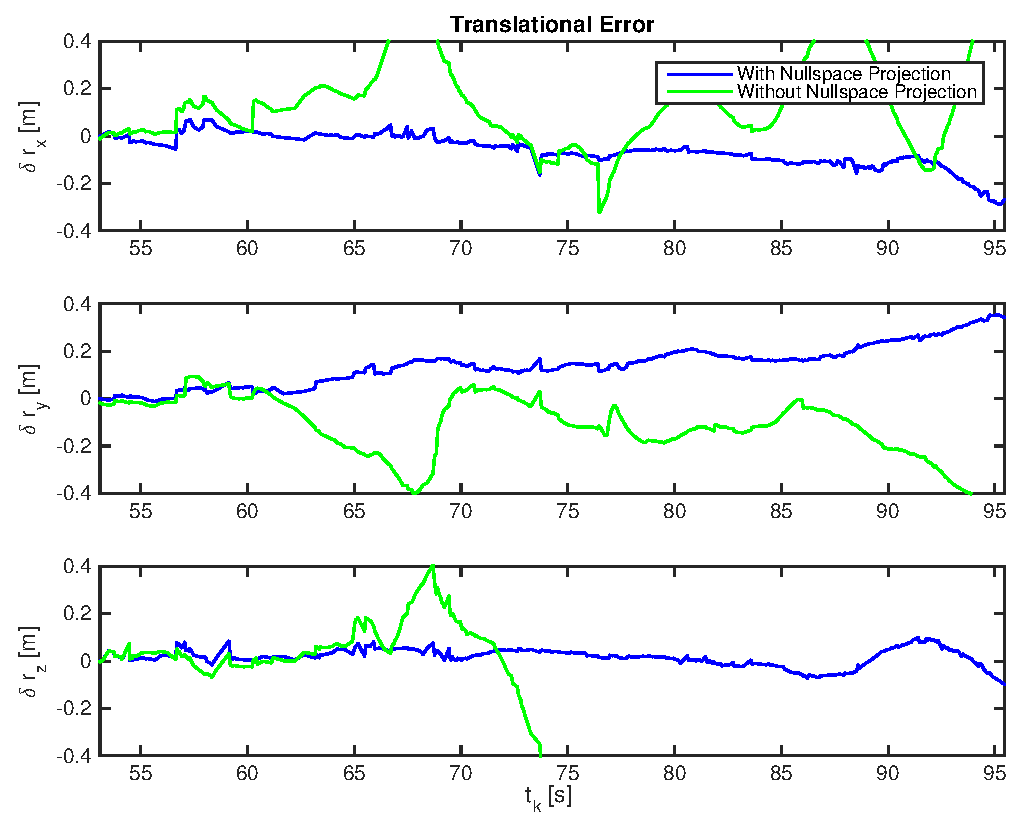
\includegraphics[width=0.48\textwidth]{figs/NST_trans}
        \label{fig:nullspace:trans_err}
    }

    \subfigure {
        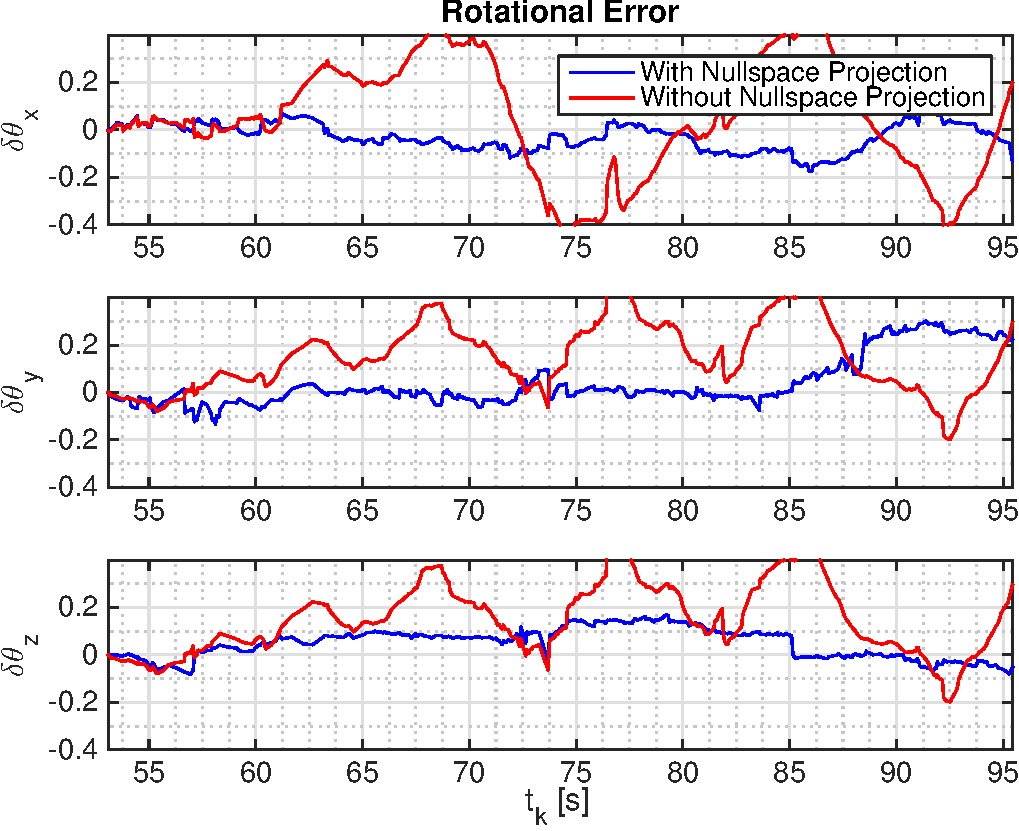
\includegraphics[width=0.48\textwidth]{figs/NST_rot}
        \label{fig:nullspace:rot_err}
    }
    
    \caption{Effect of correlation between measurement noise and filter state on MSCKF performance. The correlation between the measurement error and the state causes the filter estimates to drift further from the true values than with a modified, de-corellated measurement error.}
    \label{fig:nullspace}
\end{figure}

In order to transform $\Vec{r}^{(j)}$ into a usable form for the EKF, we can define a semi-unitary matrix $\Vec{A}$ whose columns form the basis of the left nullspace of $\Vec{H}_{f}^{(j)}$, and project $\Vec{r}^{(j)}$ into this nullspace to obtain an error equation of the correct form (to first order):
\begin{align}
    \Vec{r}_o^{(j)} := \Vec{A}^T \Vec{r}^{(j)} 
                    &\simeq \Vec{A}^T \Vec{H}_{\Vec{x}}^{(j)} \widetilde{\Vec{x}} + \Vec{0} + \Vec{A}^T \Vec{n}^{(j)} \notag \\
                    &=: \Vec{H}_{o}^{(j)} \widetilde{\Vec{x}} + \Vec{n}_o^{(j)}
\end{align}

Since $\Vec{H}_{f}^{(j)}$ has full column rank, $\Vec{A}$ has dimension $2M_j \times \left(2M_j - 3\right)$ and $\Vec{r}_o^{(j)}$ has dimension $\left(2M_j - 3\right) \times 1$.
The covariance matrix of $\Vec{n}_o^{(j)}$ is given by $\Vec{R}_o^{(j)} = \Vec{A}^T\Vec{R}^{(j)}\Vec{A}$.

We can now stack all the errors $\Vec{r}_o^{(j)}$ for all the features in the current batch to arrive at
\begin{align} \label{eq:residual_nullspace_stacked}
    \Vec{r}_o &= \Vec{H}_o \widetilde{\Vec{x}} + \Vec{n}_o .
\end{align}
The dimension of this vector can be quite large in practice, so we use the QR-decomposition of $\Vec{H}_o$ to reduce the computational complexity of the EKF update:
\begin{align}
    \Vec{H}_o = \bbm \Vec{Q}_1 & \Vec{Q}_2 \ebm \bbm \Vec{T}_\Vec{H} \\ \Vec{0} \ebm
\end{align}
where $\Vec{Q}_1, \Vec{Q}_2$ are unitary matrices and $\Vec{T}_\Vec{H}$ is an upper-triangular matrix.
Substituting this result into (\ref{eq:residual_nullspace_stacked}) and pre-multiplying by $\bbm \Vec{Q}_1 & \Vec{Q}_2 \ebm ^T$, we obtain
\begin{align}
    \bbm \Vec{Q}_1^T \Vec{r}_o \\ \Vec{Q}_2^T \Vec{r}_o \ebm &= \bbm \Vec{T}_\Vec{H} \\ \Vec{0} \ebm \widetilde{\Vec{x}} + \bbm \Vec{Q}_1^T \Vec{n}_o \\ \Vec{Q}_2^T \Vec{n}_o \ebm .
\end{align}
Noting that the quantity $\Vec{Q}_2^T \Vec{r}_o$ is only noise, we discard it and define a new error term that we use in the EKF update:
\begin{align}
    \Vec{r}_n &:= \Vec{Q}_1^T \Vec{r}_o = \Vec{T}_\Vec{H} \widetilde{\Vec{x}} + \Vec{Q}_1^T \Vec{n}_o =: \Vec{T}_\Vec{H} \widetilde{\Vec{x}} + \Vec{n}_n
\end{align} 
The covariance matrix of $\Vec{n}_n$ is given by $\Vec{R}_n = \Vec{Q}_1^T \Vec{R}_o^{(j)} \Vec{Q}_1$.

Finally, we can formulate the Kalman gain and correction equations to arrive at the updated estimates for the filter state and covariance:
\begin{align}
    \Vec{K} &= \hat{\Vec{P}}^-_{k+1}\Vec{T}_{H}^T\left(\Vec{T}_{H}\hat{\Vec{P}}^-_{k+1}\Vec{T}_{H}^T + \Vec{R}_{n} \right)^{-1} \\
    \Delta\Vec{x}_{k+1} &= \Vec{K}\Vec{r}_{n} \\
    \hat{\Vec{P}}_{k+1} &= \left(\Vec{1}_{12+6N} - \Vec{K}\Vec{T}_{H} \right)\hat{\Vec{P}}^-_{k+1}\left(\Vec{1}_{12+6N} - \Vec{K}\Vec{T}_{H} \right)^T \notag \\ 
                        &+ \Vec{K}\Vec{R}_{n}\Vec{K}^T .
\end{align}

%%%%%%%%%%%%%%%%%%%%%%%%%%%%%%%%%%%%%%%%%%%%%%%%%%%%%%%%%%%%%%%%%%%%%%%%%%%%%%%%
\section{EXPERIMENTS} \label{sec:experiments}
We compared the performance of the MSCKF and SWF algorithms on two intervals in the ``Starry Night'' dataset from the University of Toronto Institute for Aerospace Studies (UTIAS).
The dataset consists of a rigidly attached stereo camera and IMU (Figure \ref{fig:sensorhead}) observing a set of 20 features while moving along an arbitrary 3D path.
This dataset is well-suited to evaluating SLAM algorithms since accurate ground truth from a Vicon motion capture system is available for both the sensor head motion and the feature positions (Figure \ref{fig:trajectory_groundtruth}).
Since our algorithms are designed to make use of a monocular camera, we artificially blinded the stereo camera by using measurements from the left camera only.



\begin{figure}
    \centering
    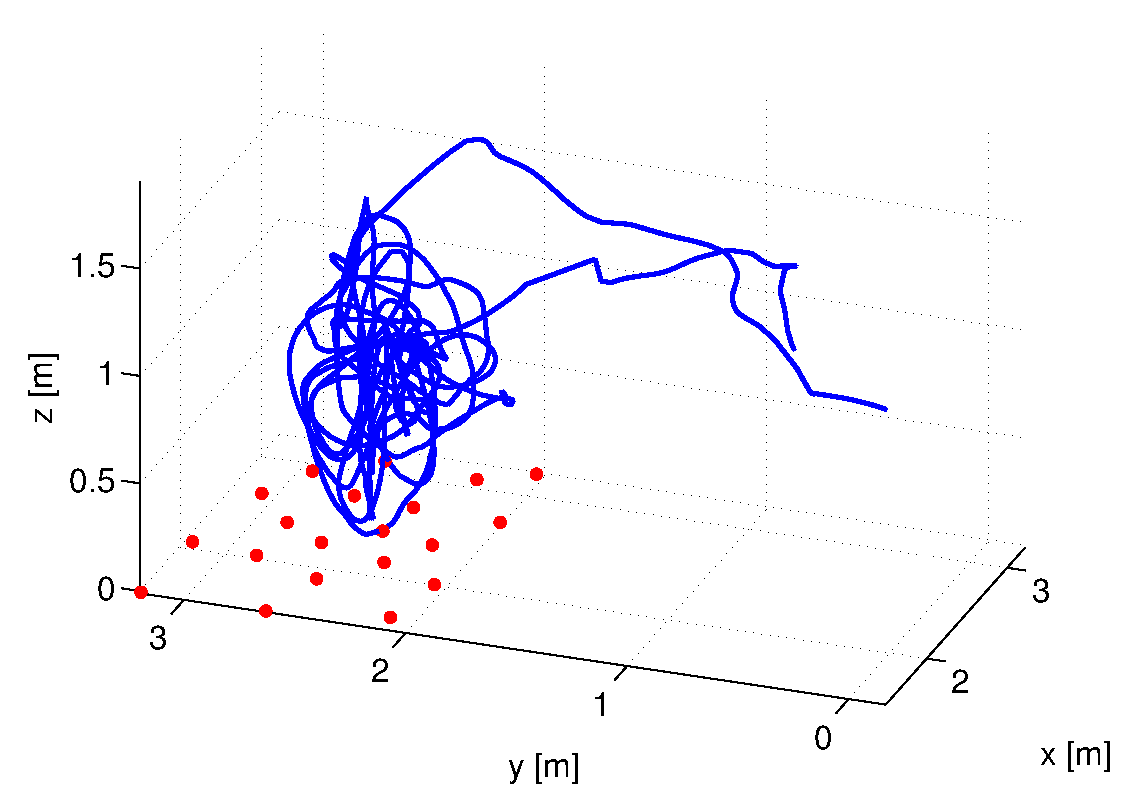
\includegraphics[width=0.48\textwidth]{figs/trajectory_groundtruth}
    \caption{Vicon ground truth for sensor head motion and feature positions in the ``Starry Night'' dataset.}
    \label{fig:trajectory_groundtruth}
\end{figure}

\subsection{Experiment 1: Many visible features}
In the first experiment, we compared the SWF and MSCKF for various parameter settings on an interval with many visible features.
Figure \ref{fig:nVisible_int1} shows the number of visible features in the first interval.
At least three features are visible in $64\%$ of this interval, and the number of visible features is frequently in excess of ten.

\begin{figure}
    \centering
    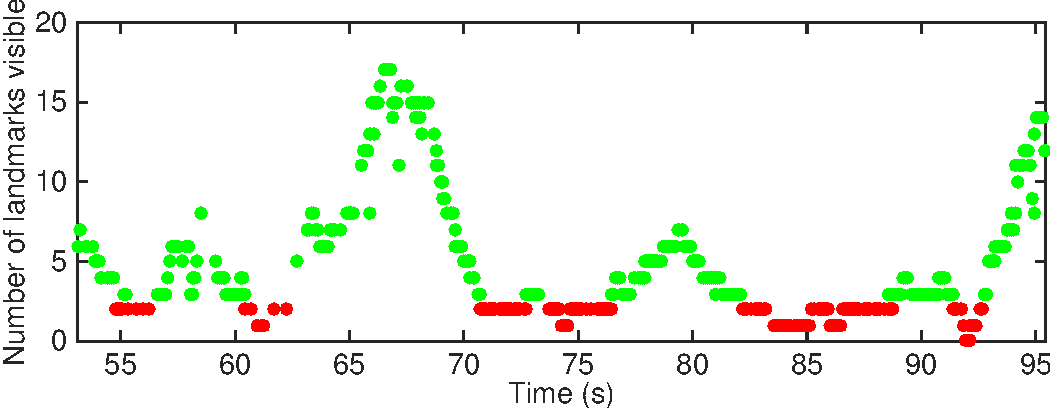
\includegraphics[width=0.48\textwidth]{figs/nVisible_500_1000}
    \caption{Number of visible features in the interval $k\in[500,1000]$. Red points indicate that fewer than three features were visible, while green points indicate at least three features were visible.}
    \label{fig:nVisible_int1}
\end{figure}

Figure \ref{fig:comp_1} shows absolute translational and rotational errors for pure IMU integration and various parameter settings for the MSCKF and SWF.
For the MSCKF, we varied both the maximum number of observations before triggering an update and the minimum number of observations for a feature track to be used in an update.
For the SWF, we varied the number of states in the sliding window.
These parameters did not significantly affect the accuracy of either filter, however Figure \ref{fig:comp_1} shows some small gains in accuracy for larger feature track lengths and window sizes.

On this interval, the SWF slightly outperforms the MSCKF in terms of translational accuracy in the $y$- and $z$-directions, and significantly outperforms the MSCKF in terms of rotational accuracy about the $x$- and $y$-axes.
The MSCKF does not perform much better than pure IMU integration on this interval, likely due to the overall low number of feature tracks in this dataset.

\begin{figure}
    \centering
    \subfigure {
        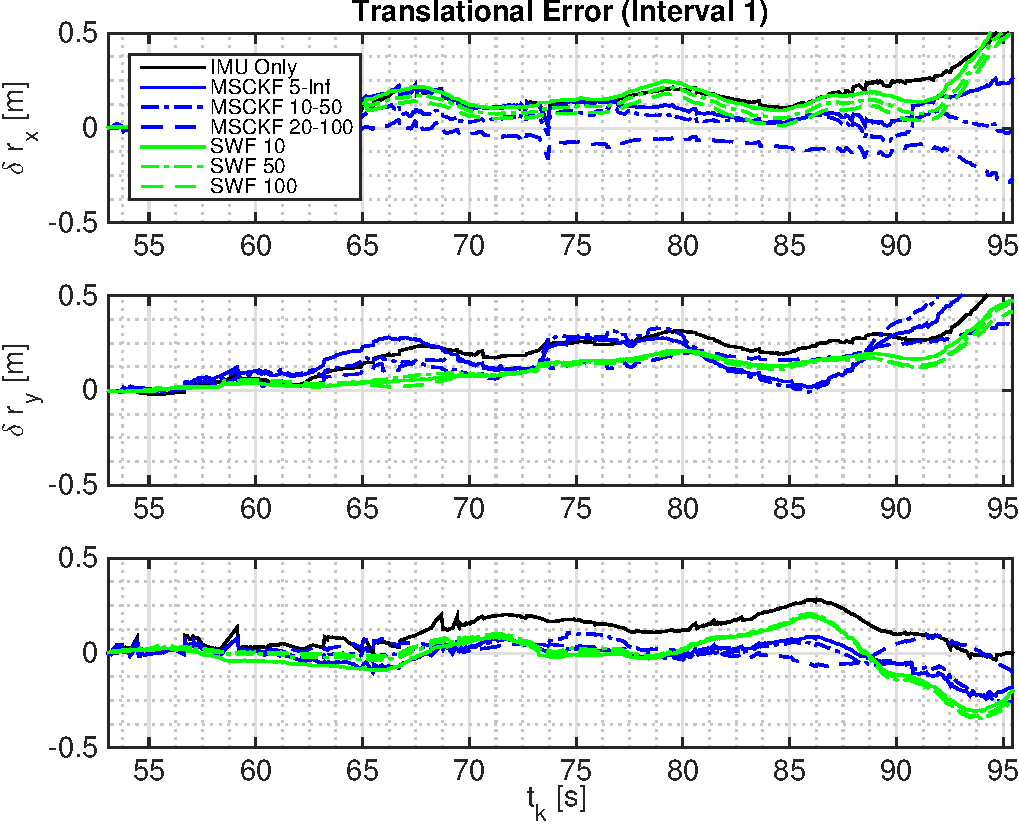
\includegraphics[width=0.48\textwidth]{figs/6-Way-Comparison-500-1000-Trans}
        \label{fig:comp_1:trans_err}
    }

    \subfigure {
        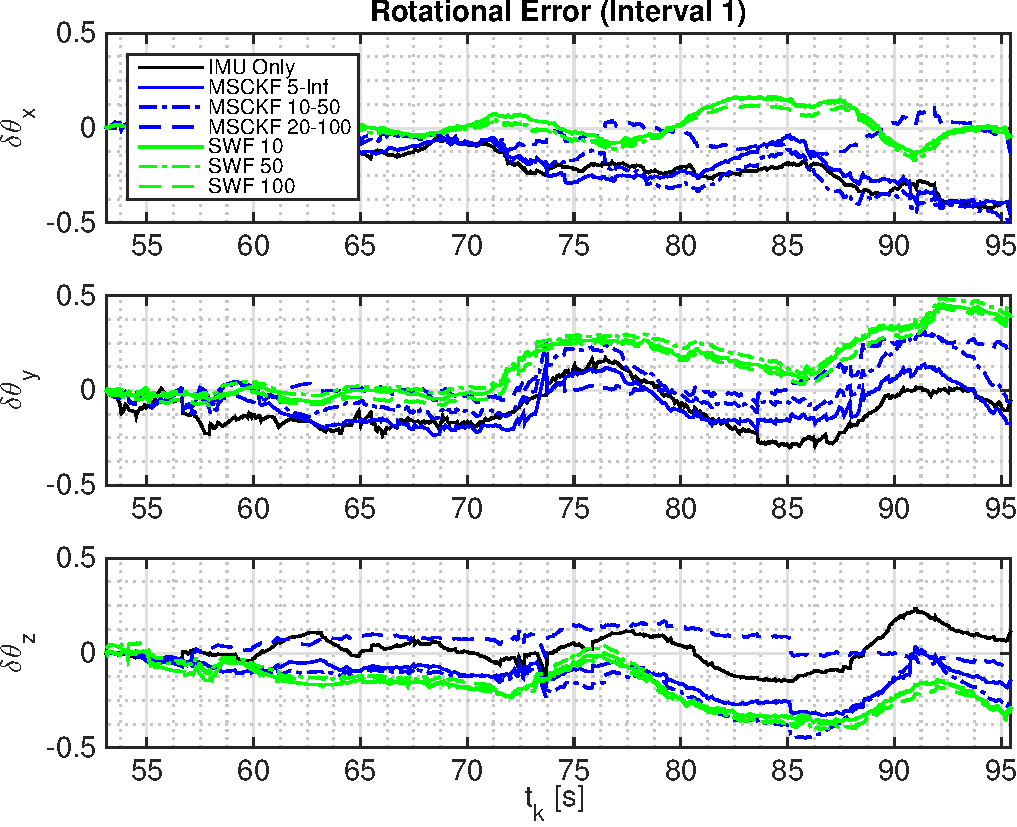
\includegraphics[width=0.48\textwidth]{figs/6-Way-Comparison-500-1000-Rot}
        \label{fig:comp_1:rot_err}
    }

    \caption{Comparison of MSCKF, SWF, and IMU integration for multiple parameter settings on the dataset interval $k\in[500,1000]$. The numbers next to ``MSCKF'' in the legend refer to the minimum and maximum feature track lengths before an EKF update is triggered, while the number next to ``SWF'' refers to the number of states in the sliding window.}
    \label{fig:comp_1}
\end{figure}


\subsection{Experiment 2: Fewer visible features}
In the second experiment, we compared the SWF and MSCKF for various parameter settings on an interval with few visible features.
Figure \ref{fig:nVisible_int2} shows the number of visible features in the second interval.
At least three features are visible in only $56\%$ of this interval, and the number of visible features rarely exceeds ten.
Moreover, the features that are visible do not remain in view of the camera for as long a time as in the first interval.

Figure \ref{fig:comp_2} shows absolute translational and rotational errors for pure IMU integration and the same MSCKF and SWF parameter settings as in Experiment 1.
Compared to Interval 1, the difference in performance between the MSCKF and SWF is less pronounced, with the exception of the SWF's clearly superior translational accuracy in the $y$-direction.
Neither filter performs substantially better than pure IMU integration on this interval, again likely due to the overall low number of feature tracks in this dataset.

\begin{figure}
    \centering
    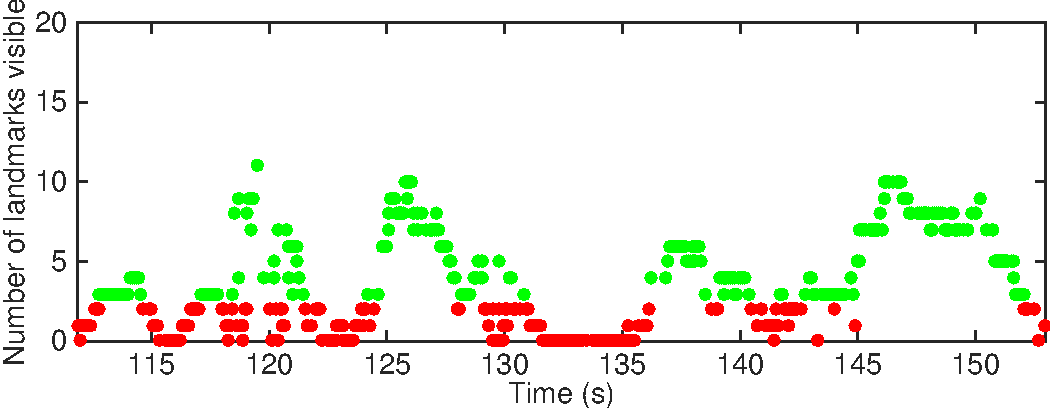
\includegraphics[width=0.48\textwidth]{figs/nVisible_1215_1715}
    \caption{Number of visible features in the interval $k\in[1215,1715]$. Red points indicate that fewer than three features were visible, while green points indicate at least three features were visible.}
    \label{fig:nVisible_int2}
\end{figure}

\begin{figure}
    \centering
    \subfigure {
        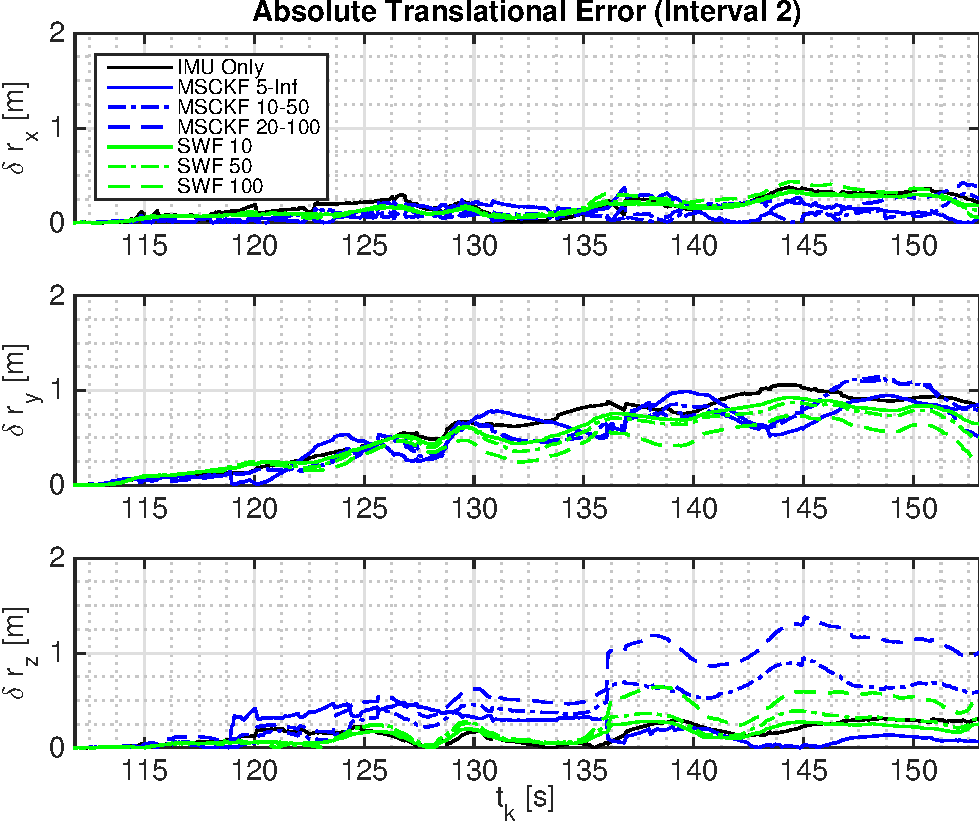
\includegraphics[width=0.48\textwidth]{figs/6-Way-Comparison-1215-1715-Trans}
        \label{fig:comp_2:trans_err}
    }

    \subfigure {
        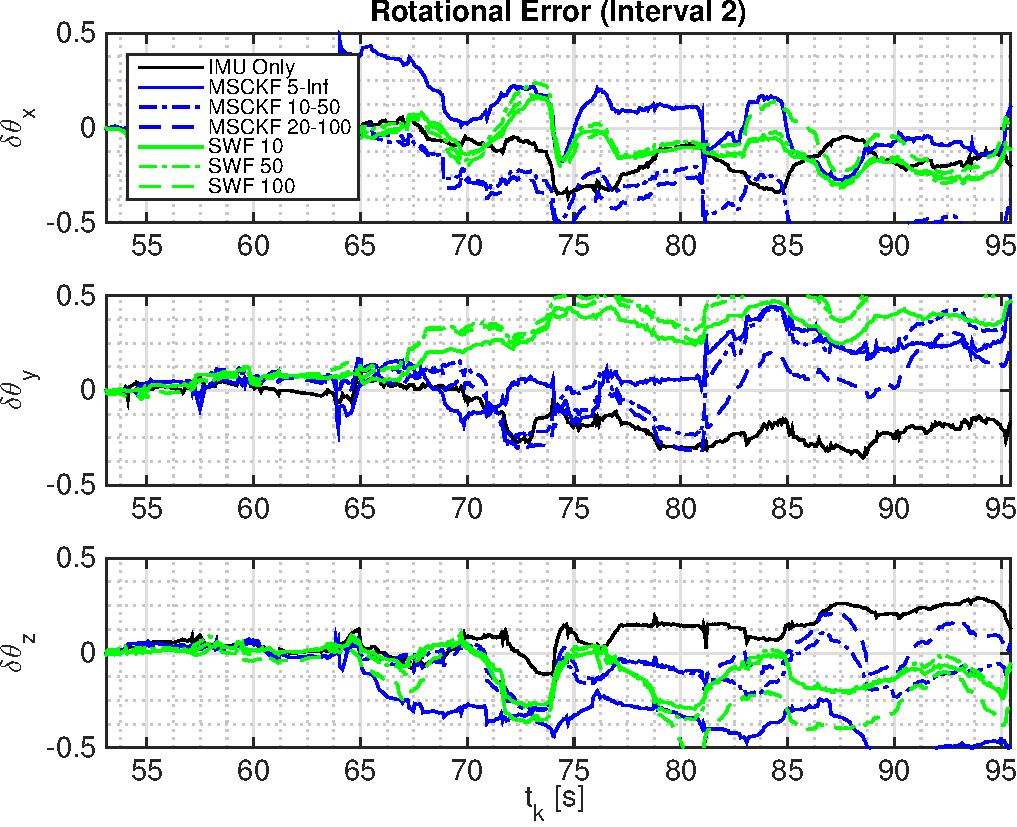
\includegraphics[width=0.48\textwidth]{figs/6-Way-Comparison-1215-1715-Rot}
        \label{fig:comp_2:rot_err}
    }

    \caption{Comparison of MSCKF, SWF, and IMU integration for multiple parameter settings on the dataset interval $k\in[1215,1715]$. The numbers next to ``MSCKF'' in the legend refer to the minimum and maximum feature track lengths before an EKF update is triggered, while the number next to ``SWF'' refers to the number of states in the sliding window.}
    \label{fig:comp_2}
\end{figure}


\subsection{Experiment 3: Effect of feature density}
In order to investigate the effect of feature density on the performance of the MSCKF and SWF, we modified the ``Starry Night'' dataset by creating synthetic feature distributions with larger spatial extents and more features than the original dataset.
We constructed each dataset so that the larger maps contained the same features as the smaller maps, plus additional features to make up the difference.
Although the camera measurements in these datasets are synthetic, the IMU data are unchanged from the original dataset.
Figure \ref{fig:trajectory_groundtruth_100lessnoisy} shows the feature distribution for the 100-feature synthetic dataset.
By generating longer feature tracks and increasing the number of features visible at each time step, these synthetic datasets allowed for a clearer comparison between the MSCKF and SWF.

\begin{figure}
    \centering
    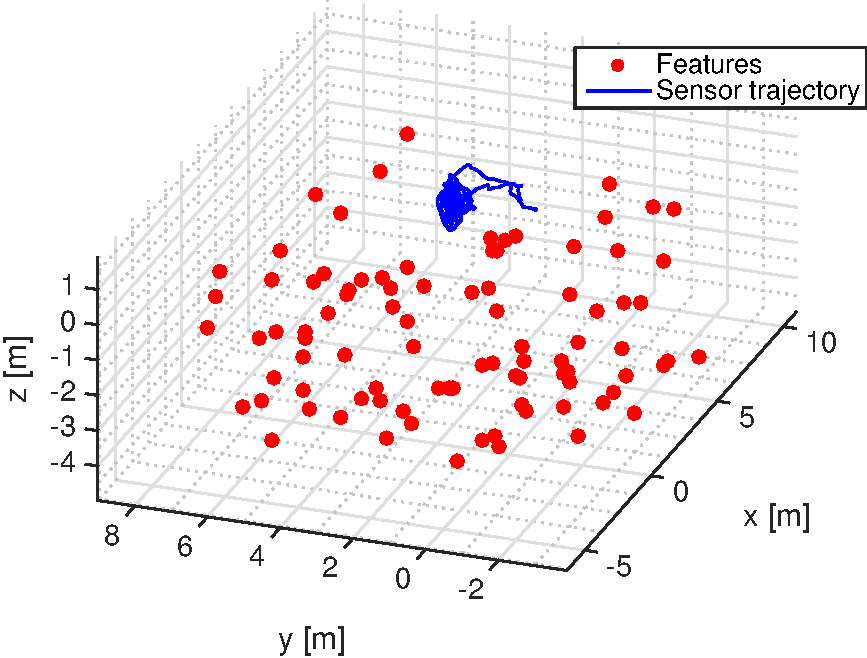
\includegraphics[width=0.48\textwidth]{figs/trajectory_groundtruth_100lessnoisy}
    \caption{Modified ``Starry Night'' dataset with 100 synthetic features. The sensor trajectory is identical to the original dataset.}
    \label{fig:trajectory_groundtruth_100lessnoisy}
\end{figure}

Figure \ref{fig:comp_3} compares translational and rotational Root Mean Squared Error (RMSE) of the MSCKF, SWF, and pure IMU integration on three synthetic datasets with 40, 60, and 100 features.
With additional features, both algorithms consistently outperform pure IMU integration, and the SWF outperforms the MSCKF by a wide margin on all three datasets.
Note that the MSCKF's performance improves as the number of features increases while the SWF's performance is not significantly affected by increasing feature count.
This result indicates that the MSCKF is much more sensitive to feature density than the SWF.

\begin{figure}
    \centering
    \subfigure {
        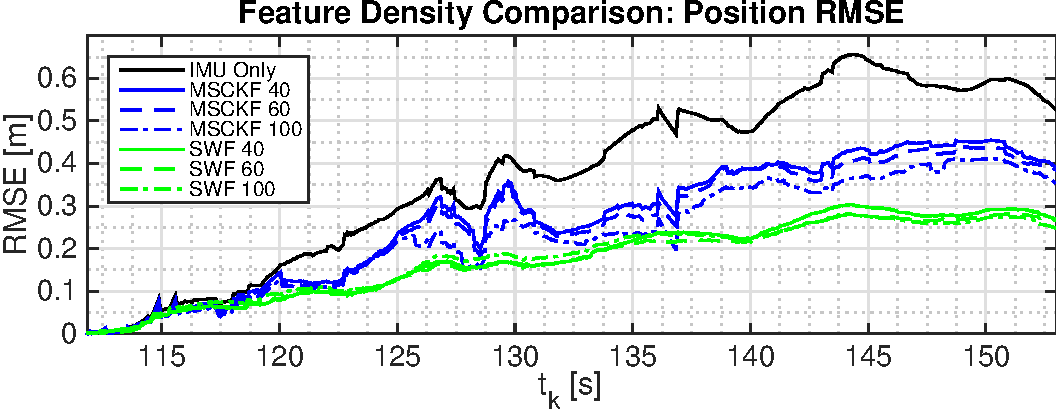
\includegraphics[width=0.48\textwidth]{figs/RMSE-Comparison-Feat-Density-1215-1715-Trans}
        \label{fig:comp_3:trans_err}
    }

    \subfigure {
        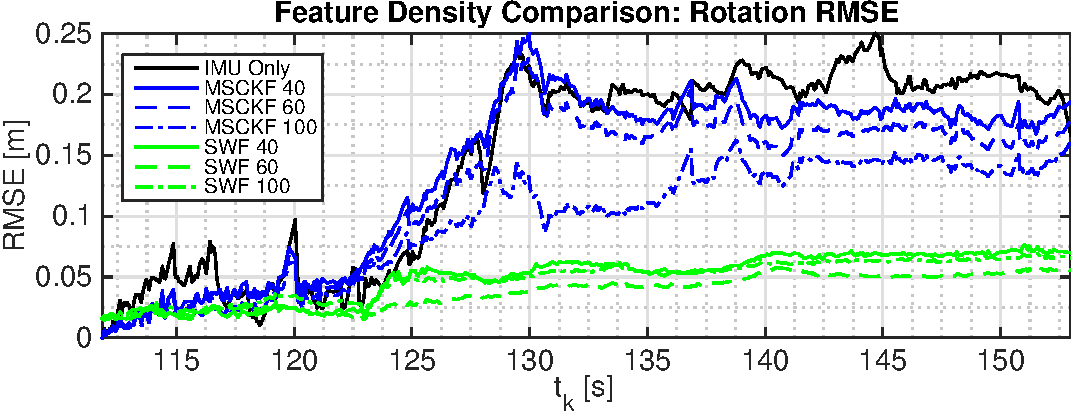
\includegraphics[width=0.48\textwidth]{figs/RMSE-Comparison-Feat-Density-1215-1715-Rot}
        \label{fig:comp_3:rot_err}
    }

    \caption{Comparison of Root Mean Squared Error (RMSE) of the MSCKF, SWF, and pure IMU integration for three different synthetic maps generated based on the IMU data in the dataset interval $k\in[1215,1715]$. The numbers next to ``MSCKF'' and ``SWF'' refer to the number of features in the dataset (40, 60 or 100).}
    \label{fig:comp_3}
\end{figure}

Table \ref{tab:rmse_nees} provides summary statistics of each algorithm's performance on the synthetic datasets.
As expected from Figure \ref{fig:comp_3}, the SWF outperforms the MSCKF in terms of average RMSE on both rotation estimation and position estimation.
It is worth noting, however, that, on average, the MSCKF achieves low Normalized Estimation Error Squared (NEES) values, which indicates that the filter scores well on consistency if not on accuracy.
The average NEES values for the SWF are substantially higher because the SWF treats each window independently and has no built-in mechanism for propagating uncertainty from window to window.
The accumulated drift error in the SWF quickly escapes the estimator's reported uncertainty envelope, and so the SWF may be considered inconsistent in the absence of a known map.

Another point in favour of the MSCKF is that the computational effort required was significantly smaller than for the SWF.
The MSCKF may therefore be better suited to vehicles with limited computational resources, particularly if they are operating in feature-rich environments.


% \begin{table*}[t]
%   \centering
%     \caption{Comparison of Average Root Mean Squared Error (ARMSE), Average Normalized Estimation Error Squared (ANEES), and Compute Time of the MSCKF and SWF on synthetic datasets.}
%   \begin{tabular}{*{11}{c}}
%               && \multicolumn{4}{c}{MSCKF} & & \multicolumn{4}{c}{SWF} \B \\ \cline{3-6} \cline{8-11}
% Feature Count && Pos. ARMSE    & Rot. ARMSE & ANEES     & Compute Time && Pos. ARMSE   & Rot. ARMSE     & ANEES & Compute Time \T\B \\ \hline
% 40            && 0.2672        & 0.1378        & 10.18  & 12.19 s      && 0.1750        & 0.0495        & 2280  & 114.3 s   \T \\
% 60            && 0.2550        & 0.1247        & 12.03  & 14.64 s      && 0.1687        & 0.0377        & 2093  & 175.9 s   \\
% 100           && 0.2304        & 0.0952        & 16.76  & 20.58 s      && 0.1755        & 0.0481        & 2013  & 245.3 s   \B \\ \hline
%   \end{tabular}
%   \label{tab:rmse_nees}
% \end{table*}

\begin{table}
    \centering
    \caption{Comparison of Average Root Mean Squared Error (ARMSE), Average Normalized Estimation Error Squared (ANEES), and Compute Time of IMU integration, MSCKF, and SWF on synthetic datasets.}
    \begin{tabular}{rlccc} 
                    &                   & \multicolumn{3}{c}{Feature Count} \B      \\ \cline{3-5}
                    &                   & 40        & 60        & 100       \T\B    \\ \hline
        IMU Only    & Position ARMSE    & 0.3679    & 0.3679    & 0.3679    \T      \\
                    & Rotation ARMSE    & 0.1452    & 0.1452    & 0.1452            \\
                    & ANEES             & 0.2850    & 0.2850    & 0.2850            \\
                    & Compute Time      & 8.90 s    & 8.90 s    & 8.90 s    \B      \\ \hline
        MSCKF       & Position ARMSE    & 0.2672    & 0.2550    & 0.2304    \T      \\
                    & Rotation ARMSE    & 0.1378    & 0.1247    & 0.0952            \\
                    & ANEES             & 10.18     & 12.03     & 16.76             \\
                    & Compute Time      & 12.19 s   & 14.64 s   & 20.58 s   \B      \\ \hline
        SWF         & Position ARMSE    & 0.1750    & 0.1687    & 0.1755    \T      \\
                    & Rotation ARMSE    & 0.0495    & 0.0377    & 0.0481            \\
                    & ANEES             & 2280      & 2093      & 2013              \\
                    & Compute Time      & 114.3 s   & 175.9 s   & 245.3 s   \B      \\ \hline
    \end{tabular}
    \label{tab:rmse_nees}
\end{table}


%%%%%%%%%%%%%%%%%%%%%%%%%%%%%%%%%%%%%%%%%%%%%%%%%%%%%%%%%%%%%%%%%%%%%%%%%%%%%%%%
\section{CONCLUSIONS} \label{sec:conclusions}
Based on our experimental results, we conclude that neither the SWF nor the MSCKF is more effective than pure IMU integration in environments with few features.
In environments with more features, both algorithms provide substantial gains over pure IMU integration, although the SWF significantly outperformed the MSCKF in terms of accuracy on the datasets we tested.
However, the accuracy of the MSCKF improves as more features are added, while the SWF is less sensitive to feature quantity.
It is unclear from these results which algorithm would perform best as the number of features grows very large.

Although the SWF appears to produce more accurate pose estimates than the MSCKF in many cases, the MSCKF has the advantage of being less computationally intensive than the SWF, and of having better consistency properties.
The MSCKF may be a better choice of algorithm in situations where computational resources are limited, or where a consistent estimate of state uncertainty is desirable.


%%%%%%%%%%%%%%%%%%%%%%%%%%%%%%%%%%%%%%%%%%%%%%%%%%%%%%%%%%%%%%%%%%%%%%%%%%%%%%%%
%%%%%%%%%%%%%%%%%%%%%%%%%%%%%%%%%%%%%%%%%%%%%%%%%%%%%%%%%%%%%%%%%%%%%%%%%%%%%%%%
%\section*{ACKNOWLEDGMENT}
%\vspace{8pt}
%%%%%%%%%%%%%%%%%%%%%%%%%%%%%%%%%%%%%%%%%%%%%%%%%%%%%%%%%%%%%%%%%%%%%%%%%%%%%%%%

\def\url#1{} % Get rid of url in citations -- also had to modify IEEEtran.bst
\bibliographystyle{IEEEtran}
\bibliography{project_bib.bib}

\end{document}
